\documentclass[13pt,oneside]{book}
\usepackage[utf8]{inputenc}
\usepackage{url}
\usepackage{graphicx}

\usepackage{geometry}
\geometry{a4paper, left=20mm, right=20mm, top=20mm, bottom=20mm}
\usepackage[margin=1.2in]{geometry}
\usepackage[toc,page]{appendix}
\usepackage{graphicx}
\usepackage{natbib}
\usepackage{lipsum}
\usepackage{caption}

\begin{document}

\captionsetup[figure]{margin=1.5cm,font=small,labelfont={bf},name={Figure},labelsep=colon,textfont={it}}
\captionsetup[table]{margin=1.5cm,font=small,labelfont={bf},name={Table},labelsep=colon,textfont={it}}
\setlipsumdefault{1}

\begin{titlepage}
\begin{center}
{\LARGE College Of Engineering Trivandrum}\\[3cm]
\linespread{1.2}\huge {\bfseries Application Software Development Lab}\\[3cm]
\linespread{1}

\includegraphics[width=5cm]{img/emblem.jpeg}\\[3cm]
{\Large GOKUL K\\ S5  CSE \\ Roll No:21\\ TVE18CS021 }\\[1cm]


\textit{ }\\[2cm]
Department of Computer Science\\[0.2cm]
\today
\end{center}

\end{titlepage}

\newpage

\begin{frame}{}
    \centering
    \hspace*{-0.5cm}
    $\vcenter{\hbox{
\includegraphics[width=1.5cm]{img/emblem.jpeg}}}$
    $\vcenter{\resizebox{0.95\textwidth}{!}{
        \begin{tabular}{c}
             CS333 - Application Software Development Lab $\cdot$ 2020 $\cdot$   \\
             \hline 
        \end{tabular}
    }}$
\end{frame}
\section*{Cycle 1}
\section*{Expt 6}
\begin{center}
    \Large{String Functions and Pattern Matching}
\end{center}

\section*{Aim}
\large To study about String Functions \& Pattern Matching.

\section*{Expiriment}
\begin{itemize}
\item 
Syntax:
\begin{verbatim}
	CREATE TABLE acct_details (
	acct_no CHAR(9) PRIMARY KEY,
	branch VARCHAR(10),
	name VARCHAR(30),
	phone VARCHAR(15)	
);
	INSERT INTO acct_details 
VALUES ('A40123401','Chicago' ,'Mike Adams' ,'(378)400-1234'),
	('A40123402','Miami','Diana George','(372)420-2345'),
	('B40123403','Miami','Diaz Elizabeth','(371)450-3456'),
	('B40123404','Atlanta','Jeoffrey George','(370)460-4567'),
	('B40123405','New York','Jennifer Kaitlyn','(373)470-5678'),
	('C40123406','Chicago','Kaitlyn Vincent','(318)200-3235'),
	('C40123407','Miami','Abraham Gottfield','(328)300-2256'),
	('C50123408','New Jersey','Stacy Williams','(338)400-5237'),
	('D50123409','New York','Catherine George','(348)500-6228'),
	('D50123410','Miami','Oliver Scott','(358)600-7230');
SELECT * FROM acct_details;
\end{verbatim}
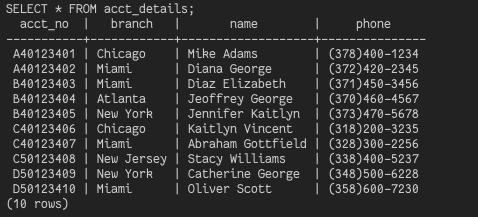
\includegraphics[]{img/p6/ss0.png}

\item
Find the names of all people starting on the alphabet 'D’.
 
Syntax:
\begin{verbatim}
SELECT name FROM acct_details
WHERE name LIKE 'D%';

\end{verbatim}
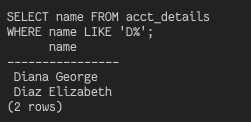
\includegraphics[]{img/p6/ss1.png}


\item
List the names of all branches containing the substring 'New’
 
Syntax:
\begin{verbatim}
SELECT branch FROM acct_details
WHERE branch LIKE '%New%';

\end{verbatim}
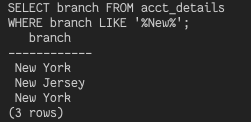
\includegraphics[]{img/p6/ss2.png}


\item
List all the names in Upper Case Format
 
Syntax:
\begin{verbatim}
SELECT UPPER(name) FROM acct_details;

\end{verbatim}
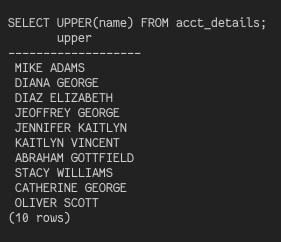
\includegraphics[]{img/p6/ss3.png}


\item
List the names where the 4th letter is 'n’ and last letter is 'n’
 
Syntax:
\begin{verbatim}
SELECT name FROM acct_details
WHERE name LIKE '___n%n';

\end{verbatim}
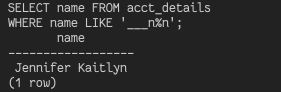
\includegraphics[]{img/p6/ss4.png}


\item
List the names starting on 'D’, 3rd letter is 'a’ and contains the substring 'Eli’
 
Syntax:
\begin{verbatim}
SELECT name FROM acct_details
WHERE name LIKE 'D_a%' and name LIKE '%Eli%';

\end{verbatim}
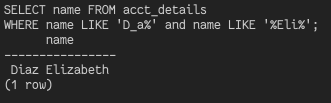
\includegraphics[]{img/p6/ss5.png}


\item
List the names of people whose account number ends in '6’.
 
Syntax:
\begin{verbatim}
SELECT name FROM acct_details
WHERE acct_no LIKE '%6';

\end{verbatim}
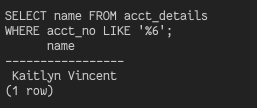
\includegraphics[]{img/p6/ss6.png}


\item
Update the table so that all the names are in Upper Case Format
 
Syntax:
\begin{verbatim}
UPDATE acct_details
SET name=UPPER(name);
SELECT * FROM acct_details;

\end{verbatim}
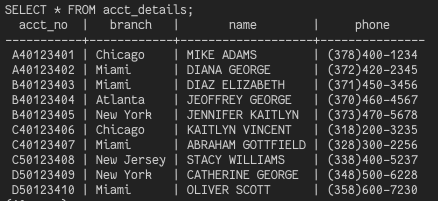
\includegraphics[]{img/p6/ss7.png}


\item
List the names of all people ending on the alphabet 't’
 
Syntax:
\begin{verbatim}
SELECT name FROM acct_details
WHERE LOWER(name) LIKE '%t';

\end{verbatim}
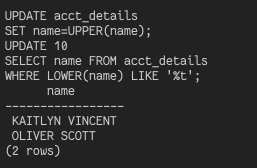
\includegraphics[]{img/p6/ss8.png}


\item
List all the names in reverse
 
Syntax:
\begin{verbatim}
SELECT REVERSE(name) AS reverse_name FROM acct_details;

\end{verbatim}
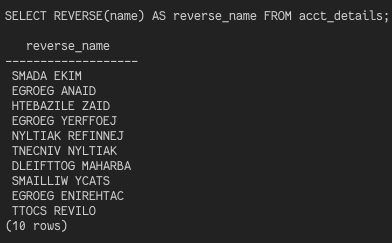
\includegraphics[]{img/p6/ss9.png}


\item
Display all the phone numbers including US Country code ( +1). For eg:
 (378)400-1234 should be displayed as +1(378)400-1234. Use LPAD function.
 
Syntax:
\begin{verbatim}
SELECT LPAD(phone, 15, '+1') FROM acct_details;

\end{verbatim}
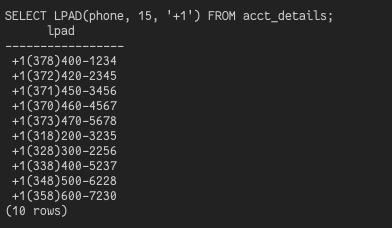
\includegraphics[]{img/p6/ss10.png}


\item
Display all the account numbers. The starting alphabet associated with the
 Account No should be removed. Use LTRIM function.
 
Syntax:
\begin{verbatim}
SELECT LTRIM(acct_no, 'ABCD') AS accnt_no, name, branch, phone
FROM acct_details;

\end{verbatim}
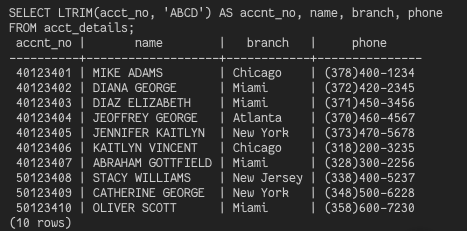
\includegraphics[]{img/p6/ss11.png}


\item
Display the details of all people whose account number starts in '4’ and name
 contains the sub string 'Williams’.

Syntax:
\begin{verbatim}
SELECT * FROM acct_details
WHERE UPPER(name) LIKE '%WILLIAMS%' or acct_no LIKE '_4%';
\end{verbatim}
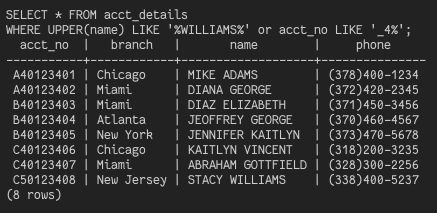
\includegraphics[]{img/p6/ss12.png}

\item
Find the reverse of the string ‘ nmutuAotedOehT’.
 
Syntax:
\begin{verbatim}
SELECT REVERSE('nmutuAotedOehT');

\end{verbatim}
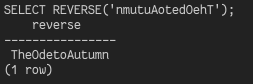
\includegraphics[]{img/p6/ss13.png}


\item
Use LTRIM function on ‘123231xyzTech’ so as to obtain the output ‘Tech’
 
Syntax:
\begin{verbatim}
SELECT LTRIM('’123231XYZTECH', '123XYZ');

\end{verbatim}
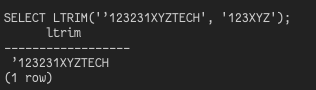
\includegraphics[]{img/p6/ss14.png}


\item
Use RTRIM function on ‘Computer ‘ to remove the trailing spaces.
 
Syntax:
\begin{verbatim}
SELECT RTRIM('Computer   ');

\end{verbatim}
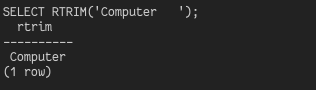
\includegraphics[]{img/p6/ss15.png}


\item
Perform RPAD on ‘computer’ to obtain the output as ‘computerXXXX’
 
Syntax:
\begin{verbatim}
SELECT RPAD('computer', 12, 'X');

\end{verbatim}
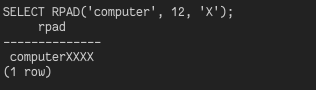
\includegraphics[]{img/p6/ss16.png}


\item
Use POSITION function to find the first occurrence of ‘e’ in the string
 ‘Welcome to Kerala’.
 
Syntax:
\begin{verbatim}
SELECT POSITION('e' in 'Welcome to Kerala');

\end{verbatim}
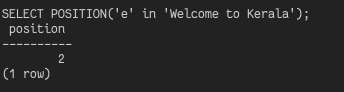
\includegraphics[]{img/p6/ss17.png}


\item
Perform INITCAP function on ‘mARKcALAwaY’.
 
Syntax:
\begin{verbatim}
SELECT INITCAP('mARKcALAwaY');

\end{verbatim}
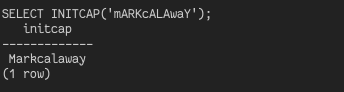
\includegraphics[]{img/p6/ss18.png}


\item
Find the length of the string ‘Database Management Systems’..
 
Syntax:
\begin{verbatim}
SELECT LENGTH('Database Management Systems');

\end{verbatim}
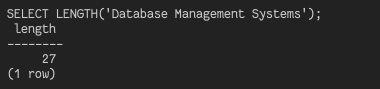
\includegraphics[]{img/p6/ss19.png}


\item
Concatenate the strings ‘Julius’ and ‘Caesar’.
 
Syntax:
\begin{verbatim}
SELECT CONCAT('Julius', 'Caesar');

\end{verbatim}
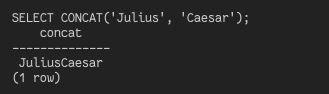
\includegraphics[]{img/p6/ss20.png}


\item
Use SUBSTR function to retrieve the substring ‘is’ from the string ‘India is
 my country’.
 
Syntax:
\begin{verbatim}
SELECT SUBSTR('India is my country', 7, 2);

\end{verbatim}
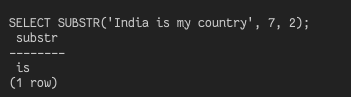
\includegraphics[]{img/p6/ss21.png}


\item
Use INSTR function to find the second occurrence of ‘k’ from the last. The
 string is ‘Making of a King’.

Syntax:
\begin{verbatim}
SELECT INSTR('Making of a King', -1, 2);

\end{verbatim}
\end{itemize}
\section*{Result}
Implemented the program for string functions and pattern matching using MariaDB 10.5 and the following output
	were obtained.
\end{document} 